\chapter{Ordered random variables}

\section{Definition}

Let $X_1,X_2,\ldots,X_n$ be a sequence of i.i.d.\ random variables. 
Suppose their distribution function is continuous.
Then there cannot be any ties i.e., for any $i\neq j$
\[
\prob*{X_i = X_j } = 0 \;.
\]
Then the $i$'th value among $X_1,\ldots,X_n$ in increasing order is
denoted by $X_{(i)}$ and is called the $i$'th \textbf{order statistic}. 
Thus 
\[
X_{(1)} < X_{(2)} < \cdots < X_{(n)}\;.
\]
In particular, $X_{(1)}$ is the minimum and $X_{(n)}$ is the maximum among $X_1,\ldots,X_n$. 

\section{Distribution of the Maximum}

Suppose $X_1$ has distribution function $F$ and density function $f$. Let $G$ denote the distribution function of $X_{(n)}$.
\[
G(x)=\prob*{X_{(n)}\leq x} = \prob*{\cap_{m=1}^n\{X_m\leq x\}} = \prod_{m=1}^n \prob*{X_m\leq x} = (F(x))^m\;.
\]
Let $g$ denote the distribution function of $X_{(n)}$. Then
\[
g(x) = G^\prime(x) = m (F(x))^{m-1} f(x) \;.
\]
For example suppose $X_1\sim\mathrm{Uniform}[0,1]$. Then $F(x)=x$ and $f(x)=1$. Therefore 
\[
g(x)=m x^{m-1} \;,
\]
which is the density function of $\mathrm{Beta}(m,1)$.

\section{Distribution of the Minimum}

Suppose $X_1$ has distribution function $F$ and density function $f$. Let $G$ denote the distribution function of $X_{(1)}$.
\[
G(x)=\prob*{X_{(1)}\leq x} = 1-\prob*{X_{(1)}>x} = 1-\prob*{\cap_{m=1}^n\{X_m>x\}} = 1-\prod_{m=1}^n \prob*{X_m>x} = 1-(1-F(x))^m\;.
\]
Let $g$ denote the distribution function of $X_{(n)}$. Then
\[
g(x) = G^\prime(x) = m (1-F(x))^{m-1} f(x) \;.
\]
For example suppose $X_1\sim\mathrm{Exponential}(1)$. Then $F(x)=1-e^{-x}$ and $f(x)=e^{-x}$. Therefore 
\[
g(x)=m e^{-mx} \;,
\]
which is the density function of $\mathrm{Exponential}(m)$ (mean $1/m$).

\section{Joint Distribution of $X_{(1)},\ldots,X_{(n)}$}

If $X_i$s have density $f$, then the joint density of $X_{(1)},\ldots,X_{(n)}$ is 
\[
n! f(x_1,x_2,\ldots,x_n) = n! f(x_1) f(x_2) \cdots f(x_n)
\]
where $x_1\leq x_2\leq \ldots\leq x_n$.

For example, suppose $X_1,X_2$ are i.i.d.\ $\mathrm{Uniform}[0,1]$ random variables. The distribution of $(X_1,X_2)$ is supported on $[0,1]\times[0,1]$ i.e., the unit square (figure on the right below). But the distribution of $(X_{(1)},X_{(2)})$ is supported on half of the unit square (figure on the left below) because $X_{(2)}$ has to be bigger than $X_{(1)}$.
\begin{figure}[h]
\begin{subfigure}{0.5\textwidth}
\centering
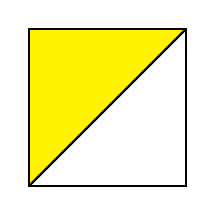
\begin{tikzpicture}[scale=2]
  \fill[yellow] (0,0) -- (1,1) -- (0,1) -- cycle;
  \draw[thick] (0,0) rectangle (1,1);
  \draw[thick] (0,0) -- (1,1);
\end{tikzpicture}
\end{subfigure}%
\begin{subfigure}{0.5\textwidth}
\centering
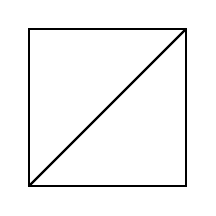
\begin{tikzpicture}[scale=2]
  \draw[thick] (0,0) rectangle (1,1);
  \draw[thick] (0,0) -- (1,1);
\end{tikzpicture}    
\end{subfigure}
\end{figure}
\noindent Consider a point in the yellow region, say $(0.4,0.8)$. If $(X_{(1)},X_{(2)})=(0.4,0.8)$ then we have two options for $(X_1,X_2)$, it can be either $(0.4,0.8)$ or $(0.8,0.4)$.
\begin{figure}[h]
\begin{subfigure}{0.5\textwidth}
\centering
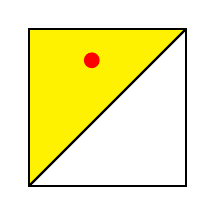
\begin{tikzpicture}[scale=2]
  \fill[yellow] (0,0) -- (1,1) -- (0,1) -- cycle;
  \draw[thick] (0,0) rectangle (1,1);
  \draw[thick] (0,0) -- (1,1);
  \fill[red] (0.4,0.8) circle [radius=0.05];
\end{tikzpicture}
\end{subfigure}%
\begin{subfigure}{0.5\textwidth}
\centering
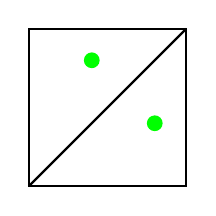
\begin{tikzpicture}[scale=2]
  \draw[thick] (0,0) rectangle (1,1);
  \draw[thick] (0,0) -- (1,1);
  \fill[green] (0.4,0.8) circle [radius=0.05];
  \fill[green] (0.8,0.4) circle [radius=0.05];
\end{tikzpicture}
\end{subfigure}
\end{figure}
\noindent Suppose we take a small set around $(0.4,0.8)$, let us denote it by $B$, in the figure it is depicted by a red ball. Corresponding to $B$ we get two regions $B_1$ and $B_2$, where $B_1$ is $B$ itself, $B_2$ is reflection of $B$. If $(X_{(1)},X_{(2)})$ belongs to $B$ then $(X_1,X_2)$ must belong to either $B_1$ or $B_2$.
\[
\prob*{(X_{(1)},X_{(2)})\in B} = 
\prob*{(X_{1},X_{2})\in B_1} + 
\prob*{(X_{1},X_{2})\in B_2} \;. 
\]
Both terms on the right are approximately
\[
A \times f(0.4)f(0.8).
\]
If $g$ is the density of $(X_{(1)},X_{(2)})$ then the term on the left is 
\[
A \times g(0.4,0.8).
\]
This shows that $g(0.4,0.8)=2 f(0.4)f(0.8)$.

\section{Joint Distribution of $X_{(i)}$ and $X_{(j)}$}

The joint density of $X_{(i)}$ and $X_{(j)}$ will be
\[
f(x_i,x_j) = \frac{n!}{(i-1)!(n-j)!} F(x_i)^{i-1} f(x_i) (F(x_i)-F(x_j))^{j-i-1} f(x_j) (1-F(x_j))^{n-j}\;.
\]
This is obtained by integrating 
\[
n!f(x_1)\cdots f(x_n)
\]
where range $x_k$ is as follows: 
if $k<i$, then $x_k$ takes values in $(-\infty,x_i]$,
if $i<k<j$, then $x_k$ takes values in $[x_i,x_j]$,
if $K>j$, then $x_k$ takes values in $[x_j,\infty)$.

For example, for $n=5,i=3,j=4$:
\begin{align*}
& 5! \int_{-\infty}^{x_3}\int_{x_1}^{x_3}\int_{x_4}^{\infty} f(x_1)f(x_2)f(x_3)f(x_4)f(x_5) dx_5dx_2dx_1  \\ 
={} & 5! f(x_3)f(x_4)\int_{-\infty}^{x_3}\int_{x_1}^{x_3}\int_{x_4}^{\infty} f(x_1)f(x_2)f(x_5) dx_1dx_2dx_5  \\
={} & 5! f(x_3)f(x_4)(1-F(x_4))\int_{-\infty}^{x_3}\int_{x_1}^{x_3} f(x_1)f(x_2) dx_1dx_2  \\
={} & 5! f(x_3)f(x_4)(1-F(x_4))\int_{-\infty}^{x_3} f(x_1)(F(x_3)-F(x_1)) dx_1  \\
={} & 5! f(x_3)f(x_4)(1-F(x_4))\int_{-F(x_3)}^{0}(-y)dy\\
\intertext{\hfill $y=F(x_3)-F(x_1)$}
={} & \frac{5!}{2} f(x_3)f(x_4)(1-F(x_4))F(x_3)^2\;.
\end{align*}

\newpage

\fancyhead[L]{\fcolorbox{red}{yellow}{Lecture 7. March 31, 2025}}
